\subsection{Ο κλασικός ημι-αθροιστής}
Ο ημι-αθροιστής είναι ένα λογικό κύκλωμα το οποίο υπολογίζει
το άθροισμα $S$ (sum) καθώς και το πιθανό κρατούμενο $C$ (carry)
που μπορεί να προκύψει από την πρόσθεση δυο bit εισόδου $a, b$.
Για να υπολογίσουμε το άθροισμα $S$ των δυο δυαδικών ψηφίων εισόδου $a, b$ πρέπει
το κύκλωμα να παράγει στην έξοδο του $1$ μονό όταν ένα από τα δυο ψηφία είναι
ίσο με $1$. Αυτό μπορεί να υλοποιηθεί με τον λογικό τελεστή της αποκλειστικής σύζευξης,
ή εν συντομία XOR.

\begin{figure}[ht]
    \centering
    \begin{tabular}{c c|c}
        $a$ & $b$ & $a \oplus b$ \\
        \hline
        0 & 0 & 0 \\
        0 & 1 & 1 \\
        1 & 0 & 1 \\
        1 & 1 & 0 \\
    \end{tabular}
    \caption{Ο πίνακας αληθείας της κλασικής λογικής πύλης XOR}
    \label{fig:1}
\end{figure}

Για τον υπολογισμό του κρατούμενου $C$ πρέπει το κύκλωμα να παράγει στην
έξοδο του $1$ αν και μόνο αν $a = b = 1$. Αυτή η έκφραση μπορεί να
υλοποιηθεί με τον τελεστή σύζευξης ΚΑΙ (AND).

\begin{figure}[ht]
    \centering
    \begin{tabular}{c c|c}
        $a$ & $b$ & $a \cdot b = a \land b$ \\
        \hline
        0 & 0 & 0 \\
        0 & 1 & 0 \\
        1 & 0 & 0 \\
        1 & 1 & 1 \\
    \end{tabular}
    \caption{Ο πίνακας αληθείας της κλασικής λογικής πύλης AND}
    \label{fig:2}
\end{figure}

Γνωρίζοντας τα επιμέρους κομμάτια μπορούμε να κατασκευάσουμε το παρακάτω
κλασικό λογικό κύκλωμα για τον ημι-αθροιστή.

\begin{figure}[ht]
    \centering
    \begin{circuitikz}
        \draw (0, 4)node[xor port] (xorone){}
        (0, 2)node[and port] (and){}
        (xorone.in 1) node[left=1cm](a) {$a$}
        (xorone.in 2) node[left=1cm](b) {$b$}
        (xorone.out) node[right=0.1cm](s) {$S = a \oplus b$}
        (and.out) node[right=0.1cm](c) {$C = a \cdot b$}
        
        (a.east) to[short,-*] (xorone.in 1) |- (and.in 1)
        (b.east) to[short,-*] ($(b.east)!.5!(xorone.in 2)$) coordinate (branch)
        -- (xorone.in 2)
        (branch) |- (and.in 2);  
    \end{circuitikz}
    \caption{Το κλασσικό κύκλωμα του ημι-αθροιστή}
    \label{fig:3}
\end{figure}

\begin{figure}[ht]
    \centering
    \begin{tabular}{c c|c c}
        $a$ & $b$ & $S = a \oplus b$ & $C = a \cdot b$ \\
        \hline
        0 & 0 & 0 & 0 \\
        0 & 1 & 1 & 0 \\
        1 & 0 & 1 & 0 \\
        1 & 1 & 0 & 1 \\
    \end{tabular}
    \caption{Ο πίνακας αληθείας του κλασικού κυκλώματος ημι-αθροιστή}
    \label{fig:4}
\end{figure}

\subsection{Ο κβαντικός ημι-αθροιστής}
Για την υλοποίησει του κβαντικού ανάλογου του ημι-αθροιστή το μόνο που
χρειάζεται να κάνουμε είναι να αντιστοιχήσουμε τις βασικές λογικές πράξεις
με τις ανάλογες κβαντικές.\\
Η λογική πύλη AND αντιστοιχεί πλήρως με την κβαντική πύλη Toffoli. Αυτό μπορούμε
να το αποδείξουμε πολύ εύκολα σχεδιάζοντας τον πίνακα αληθείας τής.

\begin{figure}[ht]
    \centering
    \includegraphics{../pdf/and.pdf}
    \caption{Το διάγραμμα της κβαντικής πύλης Toffoli}
    \label{fig:5}
\end{figure}

\begin{figure}[ht]
    \centering
    \begin{tabular}{c c c|c c c}
        $a$ & $b$ & $o$ & $a'$ & $b'$ & $o'$ \\
        \hline
        0 & 0 & 0 & 0 & 0 & 0 \\
        0 & 1 & 0 & 0 & 1 & 0 \\
        1 & 0 & 0 & 1 & 0 & 0 \\
        1 & 1 & 0 & 1 & 1 & 1 \\
    \end{tabular}
    \caption{Ο πίνακας αληθείας της κβαντική πύλης Toffoli}
    \label{fig:6}
\end{figure}

Όπως μπορούμε να διακρύνουμε οι πίνακες αληθείας είναι πανομοιότυποι με
αυτή της κλασικής πύλης AND. Επίσης το κβαντικό ανάλογο της κλασικής πύλης
XOR είναι η πύλη Feynman.

\begin{figure}[ht]
    \centering
    \includegraphics{../pdf/xor.pdf}
    \caption{Το διάγραμμα της κβαντικής πύλης Feynman}
    \label{fig:7}
\end{figure}

\begin{figure}[ht]
    \centering
    \begin{tabular}{c c|c c}
        $a$ & $b$ & $a'$ & $b'$ \\
        \hline
        0 & 0 & 0 & 0 \\
        0 & 1 & 0 & 1 \\
        1 & 0 & 1 & 1 \\
        1 & 1 & 1 & 0 \\
    \end{tabular}
    \caption{Ο πίνακας αληθείας της κβαντική πύλης Feynman}
    \label{fig:8}
\end{figure}

Γνωρίζοντας το πώς λειτουργεί ο κλασικός ημι-αθροιστής
μπορούμε να συνθέσουμε με ευκολία τον κβαντικό ημι-αθροιστή.
Έστω τα qubit εισόδου $\ket{a} = \ket{b} = \ket{0}$, θα χρειαστούμε
ένα βοηθητικό qubit $\ket{o} = \ket{0}$ το οποίο θα χρειαστεί για
τον υπολογισμό του κρατούμενου $\ket{C}$.\\

Αρχικά θα εφαρμόσουμε την πύλη Toffoli με qubit ελέγχου τα qubits
$\ket{a}, \ket{b}$ και το qubit στόχου το $\ket{o}$. Αυτή η ενέργεια
ισοδυναμεί με την λογική έκφραση $a \oplus b = C$.\\

Στο επόμενο βήμα θα εφαρμόσουμε την πύλη Feynman, με qubit-ελέγχου
το $\ket{a}$ και qubit-στόχο το $\ket{b}$. Αυτή η ενέργεια
ισοδυναμεί με την λογική έκφραση $a \cdot b = S$. Θέλουμε να επισημάνουμε
ότι αυτή η ενέργεια αλλάζει την κατάσταση του $\ket{b}_{new} = \ket{a} \cdot \ket{b}_{old}$.\\

\begin{figure}
    \centering
    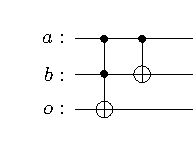
\includegraphics{../pdf/half_adder.pdf}
    \caption{Το διάγραμμα του κβαντικού-λογικού κυκλώματος του ημι-αθροιστή}
    \label{fig:9}
\end{figure}

Το τελικό διάγραμμα φαίνεται στο Σχήμα \ref{fig:9}.

